%
\documentclass[runningheads]{llncs}
%
\usepackage{graphicx}
% Used for displaying a sample figure. If possible, figure files should
% be included in EPS format.
%
% If you use the hyperref package, please uncomment the following line
% to display URLs in blue roman font according to Springer's eBook style:
% \renewcommand\UrlFont{\color{blue}\rmfamily}

\title{A CNN Based AMOLED Display Aging Compensation Quality Evaluation System\\
ECE657A Spring2020 Project Report}
\author{Alyssa Yiqin Huang, Tong Liu}
\date{15th ,August 2020}

\institute{Electrical and Computer Engineering, University of Waterloo\\
200 University Ave W, Waterloo, ON N2L 3G1, Ontario, Canada\\
\email{ yiqin.huang@uwaterloo.ca ,t344liu@uwaterloo.ca}}
\begin{document}

\maketitle              % typeset the header of the contribution
%
\begin{abstract}
An accurate and quick display luminance uniformity evaluation function plays a key feedback role for the automated AMOLED Display aging compensation evaluation system. In this report we decrepit a CNN  autoencoder based luminance uniformity evaluation system which we designed and implemented as AMOLED display aging compensation performance evaluation. Within a short period of time we are able to classify the an aged AMOLED display had a high quality compensation, a low quality compensation or had no compensation in a relatively high accuracy rate, and the system could make classification decision within 30 seconds.
\keywords{ CNN autoencoder\and AMOLED Display Aging\and AMOLED Display Aging Compensation.}
\end{abstract}

%
%
%
\section{Introduction}
AMOLED display panel has been widely used as high-end smart phone display, TV display and
automotive car informatic display. A major long-term performance issue of AMOLED display is OLED
material aging, which is the luminance performance drop at aged area cause nonuniformity issue on AMOLED display. This luminance nonuniformity shows a symptom is called burn-in see \ref{fig:1}.
To solve OLED aging issue and eliminate burn-in on AMOLED display, Ignis Innovation Inc. has developed a state of art OLED aging compensation solution to solve OLED aging problem see \ref{fig:2}.
However, to evaluate the OLED aging compensation quality is processed based on human vision. It
takes a lot of time. Its evaluations vary from person to person and difficult to compare between
evaluation results. How to evaluate the quality of OLED aging compensation with a speedy and
accurate approach is a technical challenge.
During ECE657A project, we tried to develop an OLED aging compensation evaluation function to solve above technical challenge by using the knowledge and techniques which we have learned in this course. We build a prototype system which is having conceptual functionality works as expect. The system able to classify the AMOLED display OLED aging compensation quality is GOOD or BAD. GOOD compensation quality means with OLED aging compensation, the brightness uniformity on the OLED display is beyond a certain threshold. Apparently, there will be no visible burn-in aging area on display while smart phone is normally running.BAD compensation quality means with OLED aging compensation the brightness uniformity on the OLED display is below to a certain threshold. There could be some visible burn-in area still showing on OLED display


\begin{figure}
    \centering
    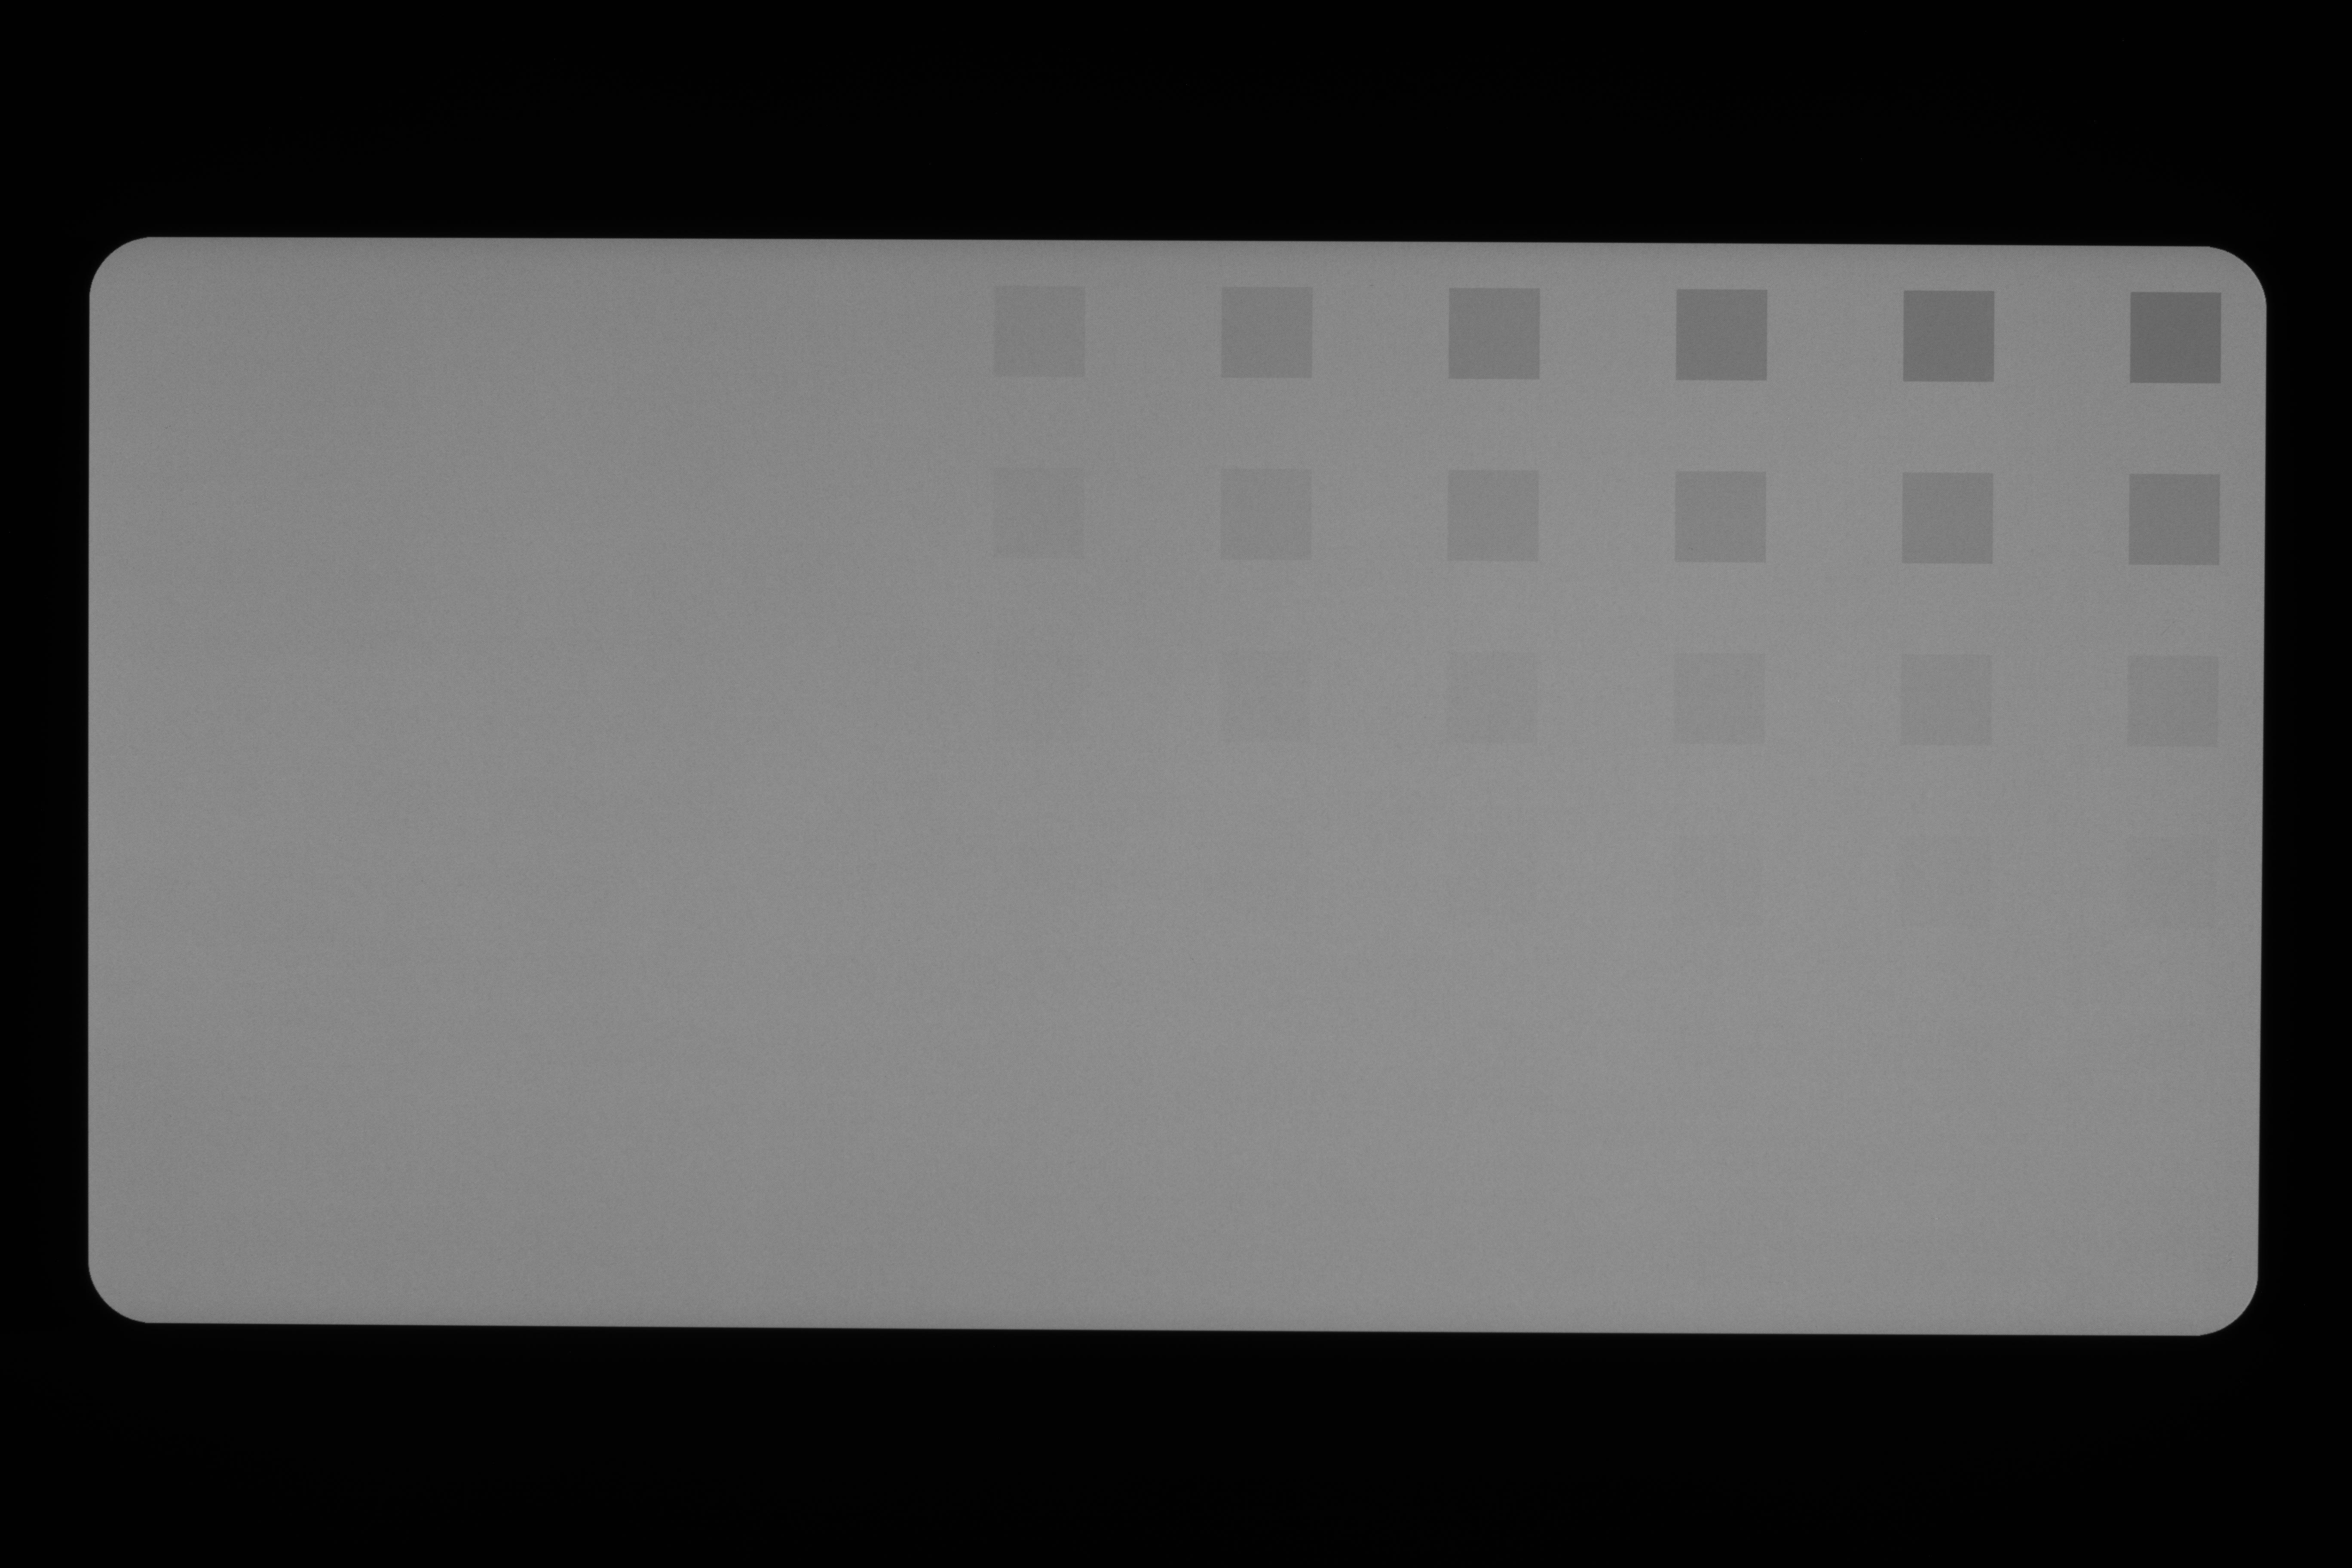
\includegraphics[width=0.3\textwidth]{uncomp.jpeg}
    \caption{An AMOLED display was aged and has OLED burn-in shown on display}
    \label{fig:1}
\end{figure}
\begin{figure}
    \centering
    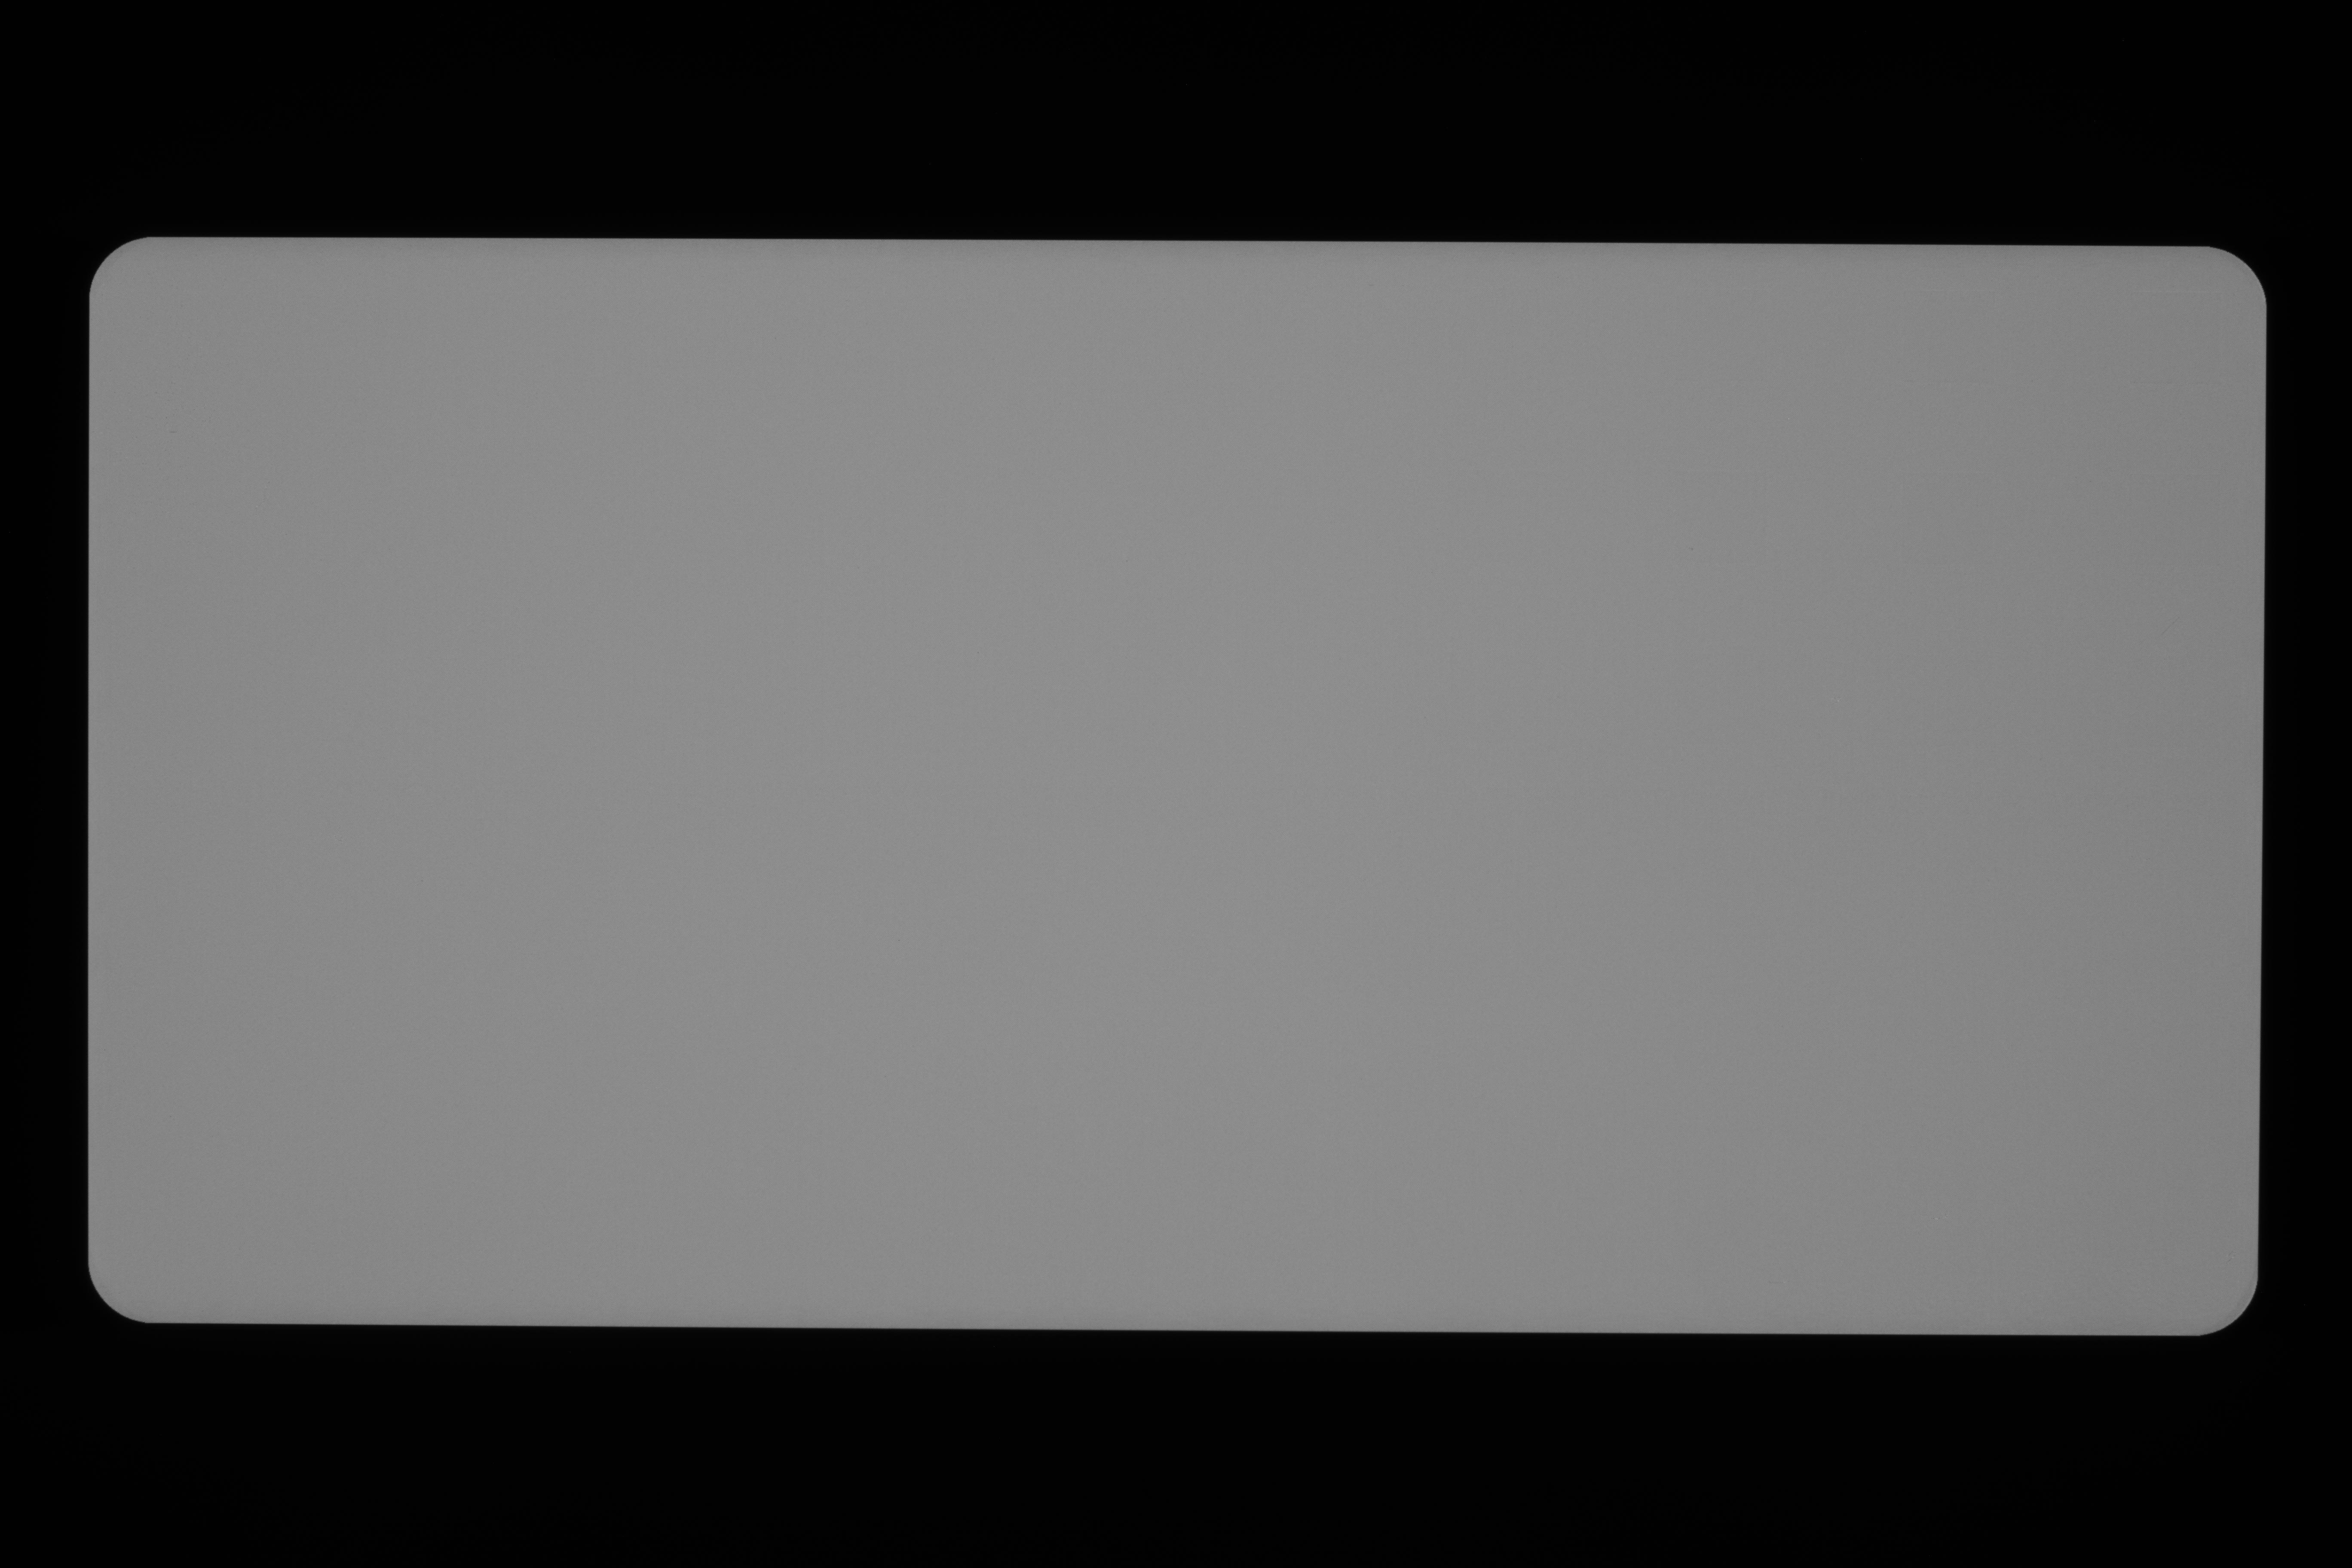
\includegraphics[width=0.3\textwidth]{comp.jpeg}
    \caption{With OLED aging compensation,the same AMOLED display's burn-in is eliminated}
    \label{fig:2}
\end{figure}

\section{Literature review}
In order to archive the project, except the materials we learned from ECE657A course, we also referenced a numbers of papers in the fields of image processing, machine learning ,deep learning and AMOLED display technologies.
Peter Barten’s research on the contrast sensitivity of human eye [10] provides a formula for contrast sensitivity which is helpful to improve accuracy of result by minimize the contrast sensitivity various of human eye. This can be done by implementing contrast sensitivity function to emphasis the difference between AMOLED display's normal areas and OLED aging areas.
Kazuki Tsutsukawa and his team at EIZO Corporation, developed an Evaluation system for Luminance Non-Uniformity Based on Deep Neural Networks. Their research paper shows that the possibility for using deep neural networks [4] to evaluate luminance non-uniformity automatically, which enables optimization of feature quantity extraction.


\end{document}
